%~~~~~~~~~~~~~~~~~~~~~~~~~~~~~~~~~~~~~~~~~~~~~~~~~~~~~~~~~~~~~~~~~~~~~
% Modelo de Teses e Dissertações CPAI: Textos ricos produzidos com Latex - v2012
% (v11)
%
%  Este modelo é trabalho de aperfeiçoamento de técnicas em Latex de:
%  Mamede Lima-Marques
%  Alfram Albuquerque
%  Alberto Magno Carvalho de Melo
%  Lauro César Araujo - laurocesar@laurocesar.com
%
%  Brasília, 19 de março de 2012
%
%~~~~~~~~~~~~~~~~~~~~~~~~~~~~~~~~~~~~~~~~~~~~~~~~~~~~~~~~~~~~~~~~~~~~~
                                                                                                                                                                                                                                                   
\documentclass[pnumplain,abnttoc,ruledheader,sumariocompleto,portuguese,twoside,openright]{report}
    
    % PACOTES GERAIS
    
    \usepackage[brazil]{babel}                 	% Determina os idiomas
	\usepackage[font=footnotesize,skip=4pt]{caption}[2011/11/10]	% captions
 	\usepackage{textcomp}						% Pacote de símbolos
 	\usepackage[T1]{fontenc}						% Seleção de códigos de fonte.
 	\usepackage{ucs}								% Usar Unicode
	\usepackage[utf8]{inputenc}					% Determina a codificação utiizada (conversão automática dos acentos)
	\usepackage[usenames,dvipsnames]{color}  	% Letras coloridas
	\usepackage{makeidx}                        % cria o indice
	\usepackage{constantes}						% pacote de constrantes
	\usepackage{teorema}                        % pacote com customizacoes deteorema 
	\usepackage{mathtools}   					% pacote matemático 
	\usepackage{dsfont}      					% matemático: simbolos de conjuntos 
	\usepackage{epigraph}    					% epigrafos no inicio dos capitulos
    \usepackage{bookmark,hyperref} 				% controlar a formação do índice
	\usepackage{multirow}						% Tabelas com células com múltiplas linhas
	\usepackage{longtable}						% Quebra de paginas em tabelas
	\usepackage{threeparttablex}					% notas no longtable
	\usepackage[nonumberlist,style=altlist]{glossaries}	% Glossario
		 			 			 		 				 		 				 			
	% PACOTES GRAFICOS
	
    \usepackage{float}							% permitir float nas figuras
    \ifx\pdfoutput\undefined
		% we are running LaTeX, not pdflatex
		\usepackage{graphicx}
	\else
		% we are running pdflatex, so convert .eps files to .pdf
		\usepackage[pdftex]{graphicx}
		\usepackage{epstopdf}
	\fi
	
	% PACOTES DE CITACOES
	
	\usepackage[brazilian,hyperpageref]{backref}	 % Paginas com as citações na bibl
	\usepackage{hyperref}						% Coloca links internos no arquivo
	\usepackage[alf]{abntcite}					% Citações padrão ABNT
	
	% Configurações do pacote backref
	\renewcommand{\backrefpagesname}				% Usado sem aopção hyperpageref de backref
		{Citado na(s) página(s): }
	\renewcommand{\backref}{}					% Texto padrão antes do número das páginas
	\renewcommand*{\backrefalt}[4]{				% Define os textos da citação
       \ifcase #1 %
         Nenhuma citação no texto.%
       \or
         Citado na página #2.%
       \else
         Citado #1 vezes nas páginas #2.%
		\fi 
	}
	
    % CONFIGURACOES DO PDF FINAL
    
     \hypersetup{
     	backref=true,
     	pagebackref=true,
		pdftitle={\meutitulo}, 
		pdfauthor={\autores - \autoresEmail},
		pdfkeywords={\palavrasChavesPortugues},
		bookmarks=true,         		% show bookmarks bar?
    		pdfsubject={\textoEpigrafe},
	    pdfproducer={Latex}, 	% producer of the document
    		colorlinks=true,       		% false: boxed links; true: colored links
    		linkcolor=blue,          	% color of internal links
    		citecolor=blue,        		% color of links to bibliography
    		filecolor=magenta,      		% color of file links
		urlcolor=blue,
		bookmarksdepth=4
		}


	% controla a pagina em branco deixada no lado par pelo twosides
	\makeatletter
	\def\cleardoublepage{
		\clearpage
		\if@twoside
			\ifodd %lado impar
				\c@page
			\else %lado par
				% imprimir texto centralizado
				\topskip0pt
				\vspace*{\fill}
					\begin{center}
						\textit{Esta página foi intencionalmente deixada em branco.}
					\end{center}
				\vspace*{\fill}
				
				% \hbox{}
	
				\thispagestyle{empty} 
				\newpage
				
				\if@twocolumn
					\hbox{}
					\newpage
				\fi
			\fi
		\fi
	}
	% \makeatothe

	% ----------------------------
	% CONTROLE DE MARGENS:
		
	% controla se as margens das páginas ímpares e pares
	% \oddsidemargin 0mm
	% \evensidemargin 0mm
	
	% controla outras margens	
	% \topmargin -10mm
	% \textwidth 16truecm
	% \textheight 24truecm
	% ----------------------------
				
	% PACOTES ADICIONAIS RECOMENDADOS:
	%\usepackage[brazil]{varioref}				% referencias ricas com \vref e \vpageref
	%\usepackage{collect}							% Coleta textos e permite reusá-los
				
				
%~~~~~~~~~~~~~~~~~~~~~~~~~~~~~~~~~~~~~~~~~~~~~~~~~~~~~~~~~~

%~~~~~~~~~~~~~~~~~~~~~~~~~~~~~~~~~~~~~~~~~~~~~~~~~~~~~~~~~~~~~~~~~~~~~
% INDICE REMISSIVO
%~~~~~~~~~~~~~~~~~~~~~~~~~~~~~~~~~~~~~~~~~~~~~~~~~~~~~~~~~~~~~~~~~~~~~

%índice
\makeindex

%~~~~~~~~~~~~~~~~~~~~~~~~~~~~~~~~~~~~~~~~~~~~~~~~~~~~~~~~~~~~~~~~~~~~~
% GLOSSÁRIO
%~~~~~~~~~~~~~~~~~~~~~~~~~~~~~~~~~~~~~~~~~~~~~~~~~~~~~~~~~~~~~~~~~~~~~

% Define a new glossary type
%\newglossary{main}{gls}{glo}{Glossário}
\makeglossaries

%~~~~~~~~~~~~~~~~~~~~~~~~~~~~~~~~~~~~~~~~~~~~~~~~~~~~~~~~~~~~~~~~~~~~~
%	MUDANÇA DE FONTES  
%	dos Capitulos e Seções para se adequar a norma ABNT
%~~~~~~~~~~~~~~~~~~~~~~~~~~~~~~~~~~~~~~~~~~~~~~~~~~~~~~~~~~~~~~~~~~~~~

\renewcommand{\ABNTchapterfont}{\bfseries\sffamily\fontseries{sbc}\selectfont}
\renewcommand{\ABNTsectionfont}{\bfseries\sffamily}

%~~~~~~~~~~~~~~~~~~~~~~~~~~~~~~~~~~~~~~~~~~~~~~~~~~~~~~~~~~~~~~~~~~~~~
%	INICIO DO DOCUMENTO
%~~~~~~~~~~~~~~~~~~~~~~~~~~~~~~~~~~~~~~~~~~~~~~~~~~~~~~~~~~~~~~~~~~~~~

\begin{document}											% inicia a classe document

\begin{sloppypar}										%

\newcounter{bbb1}										% inicia um contador
\newcounter{alf1}										% inicia um contador

%~~~~~~~~~~~~~~~~~~~~~~~~~~~~~~~~~~~~~~~~~~~~~~~~~~~~~~~~~~~~~~~~~~~~~
%     CAPA + FOLHA DE ROSTO + FOLHA DE APROVACAO + AGRADECIMENTOS
%	  TITLE + AUTHORS
%~~~~~~~~~~~~~~~~~~~~~~~~~~~~~~~~~~~~~~~~~~~~~~~~~~~~~~~~~~~~~~~~~~~~~
 
\pagenumbering{roman}									% numeração de páginas em romanos minúsculos

\newcommand{\capa}%
{%
% replacing \begin{titlepage}
\if@twocolumn
  \@restonecoltrue\onecolumn
\else
  \@restonecolfalse\newpage
\fi
\thispagestyle{empty}%
\setcounter{page}\z@
\vspace*{1cm}
\espaco{1.1}
\ABNTifnotempty{\ABNTautordata}%
  {%
  \begin{center}
    \autorformat\ABNTautordata
  \end{center}
  }
\vfill\vfill
\ABNTifnotempty{\ABNTtitulodata}%
  {%
   \begin{center}
     {\tituloformat\ABNTtitulodata\par}
   \end{center}
  }%

\vspace*{1cm}
\vfill\vfill\vfill
\begin{center}
  \begin{espacosimples}
    \setlength{\parskip}{.3cm}
    \ABNTifnotempty{\ABNTlocaldata}
      {{\localformat\ABNTlocaldata}\par}
    \ABNTifnotempty{\ABNTdatadata}
      {{\dataformat\ABNTdatadata}}
  \end{espacosimples}
\end{center}
\vspace*{1cm}
% replacing \end{titlepage} by its meaning
\if@restonecol\twocolumn \else \newpage \fi
\espaco{\ABNTespacodefault}%Corrige bug 114
}% end of \capa									% configurações da capa

\capa													% imprime a capa
\if@twoside												% cria uma página em branco
  \newpage												%  caso o twoside seja utilizado
  \thispagestyle{empty}									%  com o objetivo de manter a impressão correta
  \mbox{}
\fi

%~~~~~~~~~~~~~~~~~~~~~~~~~~~~~~~~~~~~~~~~~~~~~~~~~~~~~~~~~~~~~~~~~~~~~
%	ELEMENTOS PRE-TEXTUAIS
%	resumo - abstract - sumario - lista de fituras - lista de tabelas - lista de siglas
%	lista de abreviaturas - Introducao
%~~~~~~~~~~~~~~~~~~~~~~~~~~~~~~~~~~~~~~~~~~~~~~~~~~~~~~~~~~~~~~~~~~~~~

%
% Conforme a ABNT NBR:14724/2011, não deveria haver cabeçalhos 
% páginas nos elementos pré-textuais, mas elas deveriam ser contadas. A
% numeração começa a ser exibida nos elementos textuais. No entanto, por
% enquanto, estou usando o modelo do CPAI, que numera com algarismos romanos os
% pré-textuais.
% 

\folhaderosto											% Folha de rosto

\thispagestyle{empty}
%
% Orientações UnB:
% http://www.bce.unb.br/index.php?option=com_content&view=article&id=80&Itemid=44
%

\thispagestyle{empty}
{
\vspace*{15cm}					% Posição vertical
\footnotesize					% Tamanho da letra (igual às notas de rodapé)
\hrule							% Linha horizontal
\begin{center}					% Minipage Centralizado
\begin{minipage}[c]{12.5cm}		% Largura 
\begin{spacing}{1.0}				% Espaçamento da linha

SOBRENOME, NOME

\hspace{0.5cm} \meutituloLinhaUnica  / \autores. --
Brasília, \dataAno-

\hspace{0.5cm} 123456 p. : il. (algumas color.) ; 30 cm.
\\

\hspace{0.5cm} Orientador: \nomeOrientador
\\

\hspace{0.5cm} Dissertação (mestrado) -- Universidade de Brasília, Faculdade de
Ciência da Informação, \dataAno.
\\

\hspace{0.5cm} Bibliografia: p. 123456--7890.
\\

\hspace{0.5cm} 
	I. Arquitetura da Informação. 
	II. Lima-Marques, Mamede. 
	III. Universidade de	Brasília. 
	IV. Faculdade de Ciência da Informação. 
	V. Título 			% é assim mesmo
\\

\hspace{8.75cm} CDU 02:141:005.7
\\

\end{spacing}
\end{minipage}
\end{center}
\hrule
}				% Ficha catalográfica

\thispagestyle{empty}
%~~~~~~~~~~~~~~~~~~~~~~~~~~~~~~~~~~~~~~~~~~~~~~~~~~~~~~~~~~~~~~~~~~~~~
%
%    File      : folha_aprov
%    Type      : TeX
%    Date      : terça-feira, março 01, 2011 at 09:46
%
%    Content   : Coloque aqui sua folha de aprovação
%~~~~~~~~~~~~~~~~~~~~~~~~~~~~~~~~~~~~~~~~~~~~~~~~~~~~~~~~~~~~~~~~~~~~~

\cleardoublepage

\thispagestyle{empty}

% \begin{folhadeaprovacao}
% \end{folhadeaprovacao}
% \tipoTrabalhoCompleto sob o título \textit{``\meutituloLinhaUnica''}, defendida por
% \autores~e aprovada em \dataDefesa, em Brasília, Distrito Federal,
% pela banca examinadora constituída pelos doutores: 
% \assinatura{Prof. Dr. \nomeOrientador \\ Orientador} 
% \assinatura{Professor \\ Convidado}
% \assinatura{Professor \\ Convidado}

%-------------------------------------------------------------

% Aqui pode-se inserir, conforme a diretiva abaixo a imagem da folha de
% aprovação assinada após a banca
% use no prompt do Mac/Linux: 
%    convert fig_folha_aprovacao.jpg fig_folha_aprovacao.pdf
%
% \includepdf{imagens/fig_folha_aprovacao.pdf}
% 
% \if@twoside
% 	\mbox{}
% 	\thispagestyle{empty}
% 	\newpage
% \fi
							% Folha de aprovação

\thispagestyle{myheadings}
\addcontentsline{toc}{chapter}{Dedicatória}

\begin{flushright}

\begin{minipage}[b]{8.9cm}
\vspace{17.01cm}
Esta obra é dedicada às coisas: àquelas ínfimas e minúsculas das quais são
feitos os mundos, as estrelas, as galáxias e os universos; àquelas imensas e
colossais que moldam a beleza, consomem a morte, alimentam os sonhos,
fertilizam as ideias e iluminam o amor; às coisas que são e às que não são; às
que sentem e às que doem; às que sorriem e às que queimam; às que choram e às
divinas; às que deliram e às que dormem; às terrenas e às de Vênus\ldots~às que
existem e às que nunca existiram.\\
(Lauro César Araujo)
\end{minipage}

\end{flushright}							% Dedicatória

\thispagestyle{myheadings}
%~~~~~~~~~~~~~~~~~~~~~~~~~~~~~~~~~~~~~~~~~~~~~~~~~~~~~~~~~~~~~~~~~~~~~
%
%    File      : agradecimento
%    Type      : TeX
%    Date      : terça-feira, março 19, 2012 at 09:33
%
%    Content   : Coloque aqui seus agradecimentos.
%~~~~~~~~~~~~~~~~~~~~~~~~~~~~~~~~~~~~~~~~~~~~~~~~~~~~~~~~~~~~~~~~~~~~~

\chapter*{Agradecimentos}

Agradeço especialmente\ldots

Por fim, meu maior e mais singelo agradecimento é direcionado à Deus, por
permitir que esta incrível aventura seja possível todos os dias.

\mbox{}
\newpage						% Agradecimentos

\thispagestyle{myheadings}
%*********************************************************************
%   EPÍGRAFE
%*********************************************************************

\cleardoublepage

{\color{white}
 \chapter*{Epígrafe}
}

\begin{flushright}
\vspace{17cm}
\textit{``Não vos amoldeis às estruturas deste mundo, \\
mas transformai-vos pela renovação da mente, \\
a fim de distinguir qual é a vontade de Deus: \\
o que é bom, o que Lhe é agradável, o que é perfeito.\\
(Bíblia Sagrada, Romanos 12, 2)}
\end{flushright}
								% Epígrafe

%%%%%%%%%%%   resumo  %%%%%%%%%%%
% Ambiente para Resumo. O mesmo efeito do abstract, mas em portugues. 
%
\newcommand{\resumoname}{Resumo}
\newenvironment{resumo}%
  {%
   \if@openright\cleardoublepage\else\clearpage\fi%
   \setchaptertype{resumo}
   \pretextualchapter{\resumoname}%
   \begin{espacosimples}%
  }%
  {\end{espacosimples}\newpage}%abstract
   								% Resumo

%~~~~~~~~~~~~~~~~~~~~~~~~~~~~~~~~~~~~~~~~~~~~~~~~~~~~~~~~~~~~~~~~~~~~~
%
%    File      : abstract
%    Type      : TeX
%    Date      : terça-feira, março 19, 2012 at 10:04
%
%    Content   : Coloque aqui o resumo de sua tese/dissertação em língua estrangeira
%~~~~~~~~~~~~~~~~~~~~~~~~~~~~~~~~~~~~~~~~~~~~~~~~~~~~~~~~~~~~~~~~~~~~~

%~~~~~~~~~~~~~~~~~~~~~~~~~~~~~~~~~~~~~~~~~~~~~~~~~~~~~~~~~~~~~~~~~~~~~
%    Obrigatório, pela ABNT.
%    Versão em língua estrangeira do resumo. Obrigatório, pela ABNT. O
%    título é ABSTRACT, em inglês, RESUMEN, em espanhol castelhano, e
%    RÉSUMÉ, em francês.
%~~~~~~~~~~~~~~~~~~~~~~~~~~~~~~~~~~~~~~~~~~~~~~~~~~~~~~~~~~~~~~~~~~~~~


\begin{abstract}

The present work, conducted within the School of Brasilia,\ldots

\textbf{Key-words:} 
	\palavrasChavesIngles
\end{abstract}
 								% Abstract

% \label{label_sumario}
%\pdfbookmark{Sumário}{label_sumario}
\cleardoublepage
\pdfbookmark{\contentsname}{Contents}
\sumario 												% Sumario

\listoffigures 											% Lista de figuras

\listoftables 											% Lista de tabelas

%~~~~~~~~~~~~~~~~~~~~~~~~~~~~~~~~~~~~~~~~~~~~~~~~~~~~~~~~~~~~~~~~~~~~~
%
%    File      : lista_abrev
%    Type      : TeX
%    Date      : terça-feira, março 01, 2011 at 10:08
%
%    Content   : Coloque aqui sua lista de abreviaturas.
%~~~~~~~~~~~~~~~~~~~~~~~~~~~~~~~~~~~~~~~~~~~~~~~~~~~~~~~~~~~~~~~~~~~~~

\chapter*{Lista de Abreviaturas} 						

\begin{tabular}[t]{p{2cm} p{13.5cm}}
COBIT	& Control Objectives for Information and related
Technology \\
DIKW		& Data, Information, Knowledge, Wisdom / Dado, Informação,
Conhecimento, Sabedoria\\
ITIL		& Information Technology Infrastructure Library \\
Maia		& Método de arquitetura da informação aplicada \\
TGAI		& Teoria Geral da Arquitetura da Informação \\
TI		& Tecnologia da Informação \\
UML		& Unified Modeling Language \\
UnB		& Universidade de Brasília \\
XML		& Extensible Markup Language
\end{tabular}

%~~~~~~~~~~~~~~~~~~~~~~~~~~~~~~~~~~~~~~~~~~~~~~~~~~~~~~~~~~~~~~~~~~~~~

							% Lista de abreviaturas

%~~~~~~~~~~~~~~~~~~~~~~~~~~~~~~~~~~~~~~~~~~~~~~~~~~~~~~~~~~~~~~~~~~~~~
%	ELEMENTOS PRE-TEXTUAIS
%~~~~~~~~~~~~~~~~~~~~~~~~~~~~~~~~~~~~~~~~~~~~~~~~~~~~~~~~~~~~~~~~~~~~~

%---------------------------------------------------------------------
% INTRODUCAO
%---------------------------------------------------------------------

\chapter*{Introdução}					% O asterisco indica que o capitulo nao sera numerado

\pagenumbering{arabic}					% inicia a numeração arábica

%~~~~~~~~~~~~~~~~~~~~~~~~~~~~~~~~~~~~~~~~~~~~~~~~~~~~~~~~~~~~~~~~~~~~~
%
%    File      : introdução
%    Type      : TeX
%    Date      : terça-feira, março 19, 2012 at 10:12
%
%    Content   : Coloque aqui a introdução em de sua tese/dissertação.
%~~~~~~~~~~~~~~~~~~~~~~~~~~~~~~~~~~~~~~~~~~~~~~~~~~~~~~~~~~~~~~~~~~~~~


\label{cap_introducao}

Esta  pesquisa  pretende  mostrar  que  \ldots   através  de  \ldots
    conforme   concepçõees   apresentadas   por  [...].    Para   isso,
    articulamos o conceito de [...]  com o conceito de [...].  Fizemos
    pesquisas de recepção conforme  [...]. Articulamos os resultados a
    partir de  ideias de [...].  Neste primeiro parágrafo  você deve
    deixar  completamente claro  o  que pretende  com  o trabalho.  

    A introdução é redigida depois de escrito todo o trabalho porque,
    no decorrer da pesquisa, algumas coisas podem ser modificadas em
    relação ao projeto original.

    Depois,  de alguns parágrafos,   você  deve  falar   sobre  a
    problematização,   a   contextualização   histórica,   a   revisão
    bibliográfica,  os objetivos, a  justificativa, a  metodologia. As
    conclusões, evidentemente,  devem ficar no  capítulo Considerações
    Finais,  para  que  o  leitor  não  perca  o  interesse  pelo  seu
    trabalho.  Toda a  introdução  é feita  sem  subtítulos, em  texto
    normal.

    Tipicamente a introdução deve conter uma abordagem geral ao tema
    que justifique a razao para o trabalho ter sido desenvolvido. Deve
    resumir o estado da arte, se possível referindo outros trabalhos
    semelhantes. Os objetivos do trabalho devem estar apresentados de
    forma inequívoca e direta.
    



%---------------------------------------------------------------------
% PRIMEIRA PARTE DO TRABALHO
% objetivo geral, objetivo especifico, justificativa, metodologia, fontes
%---------------------------------------------------------------------

\part{Preparação da pesquisa}

%---------------------------------------------------------------------
% CAPÍTULOS
%---------------------------------------------------------------------

%~~~~~~~~~~~~~~~~~~~~~~~~~~~~~~~~~~~~~~~~~~~~~~~~~~~~~~~~~~~~~~~~~~~~~
%
%    File       : objetivos
%    Type       : TeX
%    Date       : terça-feira, março 01, 2011 at 10:46
%
%    Content 	: Objetivos: onde quero chegar
%~~~~~~~~~~~~~~~~~~~~~~~~~~~~~~~~~~~~~~~~~~~~~~~~~~~~~~~~~~~~~~~~~~~~~

%---------------------------------------------------------------------
\chapter{Objetivos}\label{cap_objetivos}
%---------------------------------------------------------------------

%---------------------------------------------------------------------
\section{Objetivo Geral}
%---------------------------------------------------------------------

%\objetivoGeral é definido em constantes.sty

Este trabalho tem como objetivo principal \objetivoGeral.

%---------------------------------------------------------------------
\section{Objetivos Específicos}
%---------------------------------------------------------------------

Além do objetivo geral, esta pesquisa possui ainda os seguintes objetivos
específicos:

\begin{enumerate}
  \item Fazer\ldots;
  \item Acontecer\ldots;
\end{enumerate}

%~~~~~~~~~~~~~~~~~~~~~~~~~~~~~~~~~~~~~~~~~~~~~~~~~~~~~~~~~~~~~~~~~~~~~
%
%    File      : justificativa
%    Type      : TeX
%    Date       : terça-feira, março 01, 2011 at 10:36
%
%    Content : Porque esta pesquisa é importante?
%~~~~~~~~~~~~~~~~~~~~~~~~~~~~~~~~~~~~~~~~~~~~~~~~~~~~~~~~~~~~~~~~~~~~~

%---------------------------------------------------------------------
\chapter{Justificativa}\label{cap_justificativa}
%---------------------------------------------------------------------

Conforme o \autoref{cap_ai}, 

Na justificativa deve-se considerar:


    Para justificativa deve-se procurar responder às seguintes perguntas:

       \begin{list}{--}{\leftmargin2cm\parsep0.2cm}
           \item Qual a relevância da pesquisa? 
            \item Que motivos a justificam?
            \item Quais contribuições para a compreensão, intervenção ou solução que a pesquisa apresentará?             
      \end{list}

    Processos auxiliares em uma boa justificativa:

       \begin{list}{--}{\leftmargin2cm\parsep0.2cm}
            \item[Atualidade do tema:] inserção do tema no contexto atual
            \item[Ineditismo do trabalho:] Atualidade do tema: proporcionar mais importância ao assunto.
            \item[Interesse do autor:]  vínculo do autor com o tema
            \item[Relevância do tema:] importância científica, social, educacional, etc.
            \item[Pertinência do tema:] contribuição do tema para a solução de um problema atual
      \end{list}

%~~~~~~~~~~~~~~~~~~~~~~~~~~~~~~~~~~~~~~~~~~~~~~~~~~~~~~~~~~~~~~~~~~~~~
%
%    File       : metodologia
%    Type       : TeX
%    Date       : terça-feira, março 19, 2012 at 10:32
%
%    Content 	: Metodologia utilizada para esta pesquisa
%~~~~~~~~~~~~~~~~~~~~~~~~~~~~~~~~~~~~~~~~~~~~~~~~~~~~~~~~~~~~~~~~~~~~~

%---------------------------------------------------------------------
\chapter{Metodologia}\label{metodologia}
%---------------------------------------------------------------------

%---------------------------------------------------------------------
\section{Tipo e classificação da pesquisa}
%---------------------------------------------------------------------

Baseado nas classes da ontologia\index{ontologias} de investigação científica
proposta por \citeonline[p. 151-162]{melo2010}, este trabalho possui abordagem

%---------------------------------------------------------------------
\section{Método de Pesquisa e Visão de Mundo}
%---------------------------------------------------------------------

\citeonline{van86} apresentam a disciplina de Sistemas de Informação a
partir de uma \emph{hierarquia de sistemas de investigação}, dividida em três
níveis: metanível, nível do objeto e nível da práxis\ldots


A \autoref{fig_m3hier}, traduzida por \citeonline[p. 17]{macedo2005}\ldots
%exemplo de inserção de imagem
  
\begin{figure}[htb]
\begin{center}
    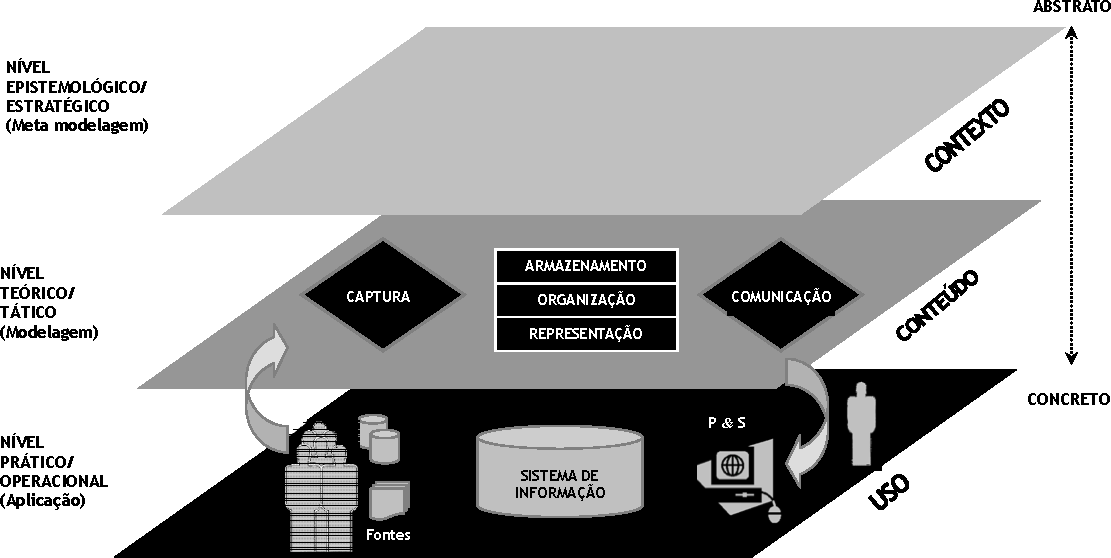
\includegraphics[scale=0.8]{imagens/fig_modeloAIMacedo.pdf}
  	\caption{\label{fig_m3hier}Metodologia de Meta-Modelagem (M{$^3$}):
  	hierarquia de sistemas de investigação}
  	\caption*{Fonte: \citeonline[p. 74]{van86}} 
\end{center} 
\end{figure}

A \autoref{tab-nivinv}\ldots

\begin{table}[htb]
\footnotesize
\caption[Níveis de investigação]{\footnotesize{Níveis de investigação.
\cite{van86}}}
\label{tab-nivinv}
\begin{tabular}{p{2.6cm}|p{6.0cm}|p{2.25cm}|p{3.40cm}}
  %\hline
   \textbf{Nível de Investigação} & \textbf{Insumos}  & \textbf{Sistemas de Investigação}  & \textbf{Produtos}  \\
    \hline
    Meta-nível & Filosofia da Ciência  & Epistemologia & Paradigma  \\
    \hline
    Nível do objeto & Paradigmas do metanível e evidências do nível inferior &
    Ciência  & Teorias e modelos \\
    \hline
    Nível inferior & Modelos e métodos do nível do objeto e problemas do nível inferior & Prática & Solução de problemas  \\
   % \hline
\end{tabular}
\end{table}


%---------------------------------------------------------------------
\section{Fontes de pesquisa} \label{metodologiaFontes}
%---------------------------------------------------------------------

A revisão da literatura foi realizada principalmente nas --- mas não limitada às
--- fontes seguintes:

\textbf{Bancos de Testes e Dissertações}

\begin{list}{--}{\parsep0.0cm\leftmargin2.0cm}
  \item Banco de Teses da CAPES (\url{http://www.capes.gov.br/servicos/banco-de-teses/});
  \item Banco de Teses e Dissertações da UnB (\url{http://bce.unb.br/});
\end{list}

\textbf{Bases de Dados}

\begin{list}{--}{\parsep0.0cm\leftmargin2.0cm}
  \item ACM Digital Library (\url{http://dl.acm.org/});
  \item Periódicos CAPES (\url{http://www.periodicos.capes.gov.br/})
  \item ProQuest (\url{http://search.proquest.com/})
  \item School of Information (\url{http://www.ischool.utexas.edu/});
  \item Web of Knowledge (\url{http://wok.mimas.ac.uk/});
  \item \ldots
\end{list}

\textbf{Periódicos}

\begin{list}{--}{\parsep0.0cm\leftmargin2.0cm}
  \item Ciência da Informação (IBICT);
  \item Journal of the American Society for Information Science and Technology
  (JA-SIST);
\end{list}

%---------------------------------------------------------------------
%---------------------------------------------------------------------
\subsection{Bibliometria}\label{metodologiaBibliometria}
%---------------------------------------------------------------------

A \autoref{tab_bibliometria_termosInformationConfig} contém dados bibliométricos
de pesquisas de termos chaves em algumas das bases de dados listadas na
\autoref{metodologiaFontes}\ldots

% EXEMPLO DE LONG TABLE
% INFORMATION e CONFIGURATION - Tabela principal de consultas de
\begin{center}
\footnotesize{
\begin{ThreePartTable}

\begin{longtable}{p{7.2cm}|p{6.3cm}|p{1.8cm}}

\caption[Resultados obtidos na consulta de termos ``configuration'' e
``information'' em bases de dados em 29.1.2012.]{\footnotesize{Resultados obtidos
na consulta de termos ``configuration'' e ``information'' em bases de dados.
Consultas realizadas em 29.1.2012. Período pesquisado: todos disponíveis nas
bases.}}
\label{tab_bibliometria_termosInformationConfig}
\\

%This is the header for the first page of the table...
\hline 
\textbf{Base de dados}	& \textbf{Termos e critérios} & \textbf{Resultados} \\
\hline 
%\endfirsthead
\endhead

%This is the footer for all pages except the last page of the table...
  \multicolumn{3}{r}{{Continua\ldots\ldots}} \\
\endfoot

%This is the footer for the last page of the table...
\hline \hline
\endlastfoot

%Now the data...

    % ``information configuration''
	\multirow{2}{*}{Academic Search Premier - ASP (EBSCO)}\tnote{a}
	& Titulo=(``information configuration'')
	& 1\tnote{b}
	\\
	& Titulo=(``configuration of information'')
	& 1\tnote{e}	
	\\ \hline	

	\multirow{2}{*}{Cambridge Journals Online}\tnote{a}
	& Titulo=(``information configuration'')
	& 0
	\\
	& Titulo=(``configuration of information'')
	& 0
	\\ \hline	

	\multirow{2}{*}{Highwire Press}\tnote{a}
	& Titulo=(``information configuration'')
	& 0
	\\
	& Titulo=(``configuration of information'')
	& 0
	\\ \hline	

	\multirow{2}{*}{Nature (NPG)}\tnote{a}
	& Titulo=(``information configuration'')
	& 0
	\\
	& Titulo=(``configuration of information'')
	& 0
	\\ \hline	

	\multirow{2}{*}{Oxford Journals (Oxford University Press)}\tnote{a}
	& Titulo=(``information configuration'')
	& 0
	\\
	& Titulo=(``configuration of information'')
	& 0
	\\ \hline	

	\multirow{3}{*}{SciELO.ORG}\tnote{a}
	& Titulo=(``information configuration'')
	& 0
	\\
	& Titulo=(``configuration of information'')
	& 0
	\\
	& Title: ``configuração da informação''
	& 0
	\\ \hline	

	\multirow{2}{*}{Science (AAAS)}\tnote{a}
	& Titulo=(``information configuration'')
	& 0
	\\
	& Titulo=(``configuration of information'')
	& 0
	\\ \hline	

	\multirow{2}{*}{ScienceDirect (Elsevier)}\tnote{a}
	& Titulo=(``information configuration'')
	& 0
	\\
	& Titulo=(``configuration of information'')
	& 0
	\\ \hline	

	\multirow{2}{*}{SpringerLink (MetaPress)}\tnote{a}
	& Titulo=(``information configuration'')
	& 0
	\\
	& Titulo=(``configuration of information'')
	& 0
	\\ \hline	

	\multirow{2}{*}{E-LIS}
	& Title: ``information configuration''
	& 2\tnote{c}
	\\
	& Title: ``configuration of information''
	& 1\tnote{d}
	\\ \hline	

	\multirow{2}{*}{Web of Knowledge}
	& Title: ``information configuration''
	& 0
	\\
	& Title: ``configuration of information''
	& 0
	\\ \hline	
	
\end{longtable}

	\begin{tablenotes}
		\item [a] Base de Periódicos CAPES.
		\item [b] O único texto obtido \ldots
		\item [c] Os textos recuperados \cite{hammer2005} e \cite{apps2001} se
		referem, respectivamente, a um manual de uso de uma ferramenta de
		gerenciamento de informação para bibliotecários e a um serviço baseado em Dublincore.
		\item [d] O único texto obtido \ldots
		\item [e] O único texto obtido \ldots

	\end{tablenotes}
	
\end{ThreePartTable}
}
\end{center}


% Figura - Web of Science 1 - Detalhamento
\begin{figure}[htb]
\begin{center}
  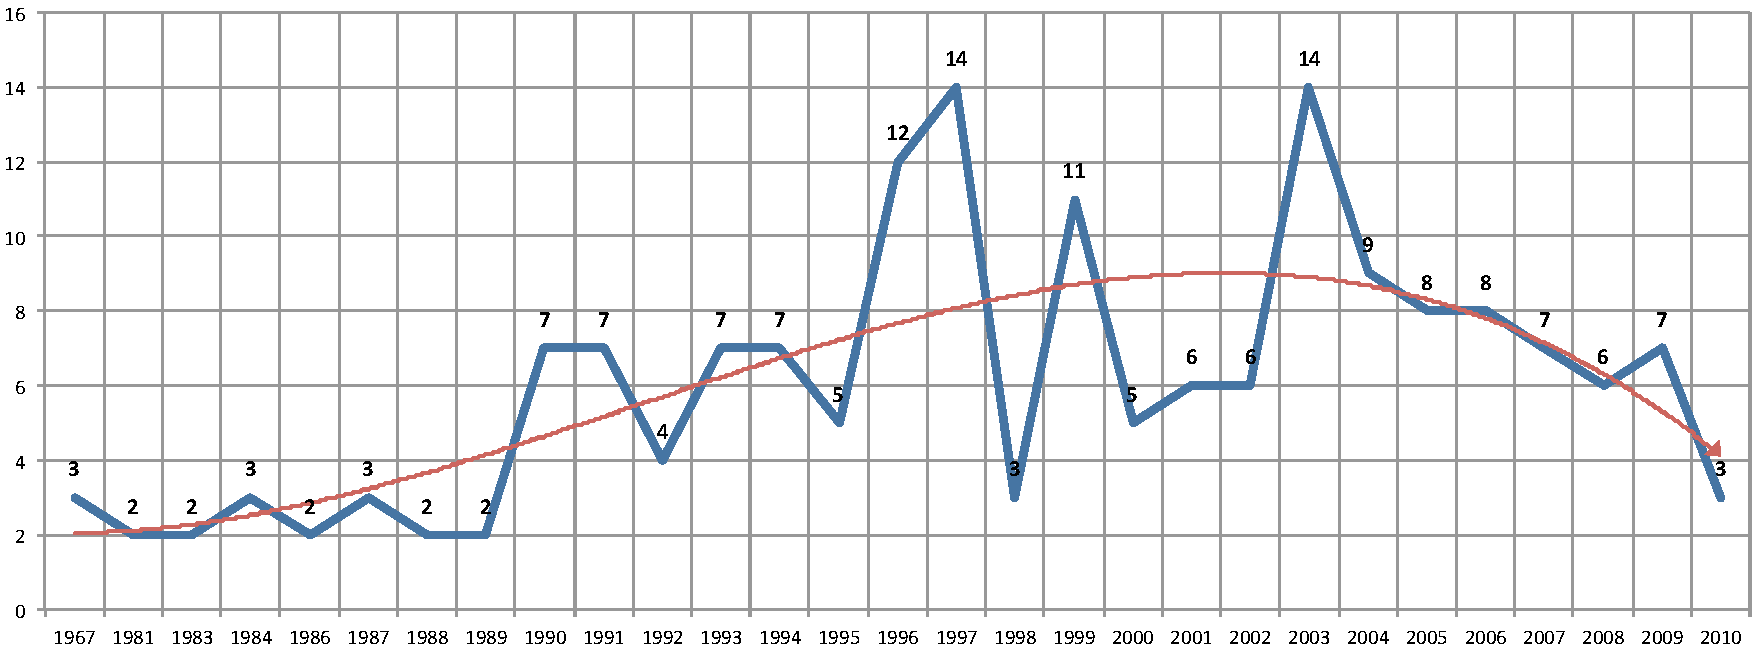
\includegraphics[scale=0.55]{imagens/bibliometriaWebOfScience1.pdf}
  \caption{\label{fig_biblioWebOfScience1}Bibliometria - Web of Science -
  Detalhamento da consulta - Critério: Title=(``configuration management'').}
  \caption*{Fonte: autores}
\end{center}
\end{figure}


%---------------------------------------------------------------------


%---------------------------------------------------------------------
% SEGUNDA PARTE DO TRABALHO
% revisao da literatura - fundamentos
%---------------------------------------------------------------------

\part{Revisão de Literatura e Fundamentos}

\chapter*{Prólogo}

Nesta parte do texto são expostos\ldots

Cada um desses tópicos são encontrados nos capítulos da seguinte maneira:

\begin{list}{--}{\parsep0.0cm\leftmargin2.0cm} 

  \item \textbf{\autoref{resultadoAIRei} - \nameref{resultadoAIRei}}: aborda\ldots

  \item \ldots 
  
\end{list}

%---------------------------------------------------------------------
% CAPITULOS
%---------------------------------------------------------------------

%------------------------------------------------
\chapter{Revisão 1} \label{cap_ai}
%------------------------------------------------

%------------------------------------------------
\section{Introdução}
%------------------------------------------------

Neste capítulo \ldots


%------------------------------------------------
\section{Seção sobre isso}
%------------------------------------------------

%------------------------------------------------
\section{Seção sobre aquilo}
%------------------------------------------------

Neste capítulo \ldots

%------------------------------------------------
\section{Seção sobre queijo}
%------------------------------------------------

Neste capítulo \ldots

%------------------------------------------------
\section{Seção sobre pamonha}
%------------------------------------------------

Neste capítulo \ldots

%------------------------------------------------
\section{Seção sobre milho cozinho com sal e águla}
%------------------------------------------------

Neste capítulo \ldots

%------------------------------------------------
\section{Conclusão}
%------------------------------------------------

Neste capítulo \ldots




%---------------------------------------------------------------------
% TERCEIRA PARTE DO TRABALHO
% resultados
%---------------------------------------------------------------------

\part{Resultados}

%---------------------------------------------------------------------
% CAPITULOS
%---------------------------------------------------------------------

\chapter{Resultado 1}
\label{cap_resultadoAI}

%-----------------------------
\section{Introdução}
%-----------------------------

Este capítulo apresenta \ldots

A \autoref{resultadoAIRei} apresenta\ldots

%-----------------------------
\section{Título AI e o rei}\label{resultadoAIRei}
%-----------------------------



%---------------------------------------------------------------------
% CONSIDERACOES FINAIS
%---------------------------------------------------------------------

%finaliza a parte
\bookmarksetup{startatroot}% this is it
\addtocontents{toc}{\bigskip}% perhaps as well

%Considerações finais

%~~~~~~~~~~~~~~~~~~~~~~~~~~~~~~~~~~~~~~~~~~~~~~~~~~~~~~~~~~~~~~~~~~~~~
%
%    File       : conclusão
%    Type       : TeX
%    Date       : terça-feira, março 01, 2011 at 10:57
%
%    Content 	: Considerações gerais sobre a pesquisa e o resultado
%~~~~~~~~~~~~~~~~~~~~~~~~~~~~~~~~~~~~~~~~~~~~~~~~~~~~~~~~~~~~~~~~~~~~~

%---------------------------------------------------------------------
\chapter{Considerações finais}\label{cap_conclusao}
%---------------------------------------------------------------------

Este trabalho\ldots

%---------------------------------------------------------------------
\section{Contribuições e alcance dos objetivos}
\label{conclusao_contribuicoes}
%---------------------------------------------------------------------

Nesta seção estão listadas, na ordem em que apareceram no texto, algumas das
contribuições mais importantes desta pesquisa.

\begin{list}{--}{\leftmargin2cm\parsep0.2cm}

    \item Derivações jklfgjklfjd;

    \item Modelos e Métodos para klfkjfls;d;

    \item Estudos de casos jffdjsfdsj;

    \item Elaboração de modelos de operacionalização jjfdjskjk;

    \item Avaliação de impacto jkflsdl; e,

    \item Modelo de comunicação jfdjfsdjklj.

\end{list}

%---------------------------------------------------------------------
\section{Possibilidades de pesquisas futuras}\label{conclusaoTrabalhosFuturos}
%---------------------------------------------------------------------

\begin{list}{--}{\leftmargin2cm\parsep0.2cm}

    \item Derivações jklfgjklfjd;

    \item Modelos e Métodos para klfkjfls;d;

    \item Estudos de casos jffdjsfdsj;

    \item Elaboração de modelos de operacionalização jjfdjskjk;

    \item Avalição de impacto jkflsdl; e,

    \item Modelo de comunicação jfdjfsdjklj.

\end{list}

%~~~~~~~~~~~~~~~~~~~~~~~~~~~~~~~~~~~~~~~~~~~~~~~~~~~~~~~~~~~~~~~~~~~~~
%	ELEMENTOS PÓS-TEXTUAIS
%~~~~~~~~~~~~~~~~~~~~~~~~~~~~~~~~~~~~~~~~~~~~~~~~~~~~~~~~~~~~~~~~~~~~~


%---------------------------------------------------------------------
% REFERENCIAS - bibliografia
%---------------------------------------------------------------------
\bibliography{bib/referencias}

% ---------------------------------------------------------------------
% GLOSSÁRIO
% ---------------------------------------------------------------------
% Não utilize ponto (.) no final das frases. Ele é adicionado automaticamente
%
% Para compilar o glossario, digite no prompt:
%    makeglossaries main.tex
% Recompile o projeto
% 

\newglossaryentry{palavraChave1}{ 
	name={nome no singular},
	plural={nome no plural},
	description={conjunto de \glspl{produto} ou de \glspl{itemConfiguracao} que
	juntos possuem uma fronteira bem definida de tal forma que se tornam um item
	individual de configuração. São partes de produtos finais ou de
	outros componentes} }

\newglossaryentry{produto}{ 
	name={produto},
	plural={produtos},
	description={produto é o resultado de um processo} }

\newglossaryentry{itemConfiguracao}{ 
	name={item de configuração},
	plural={itens de configuração},
	description={conjunto de \glspl{produto} no plural ou de \gls{produto} no
	singular} }

\glsaddall
\renewcommand{\glossaryname}{Glossário} 
\renewcommand{\glossarypreamble}{Este glossário\ldots}

%Traduções para o ambiente glossaries
\providetranslation{Glossary}{Glossário}
\providetranslation{Acronyms}{Siglas}
\providetranslation{Notation (glossaries)}{Notação}
\providetranslation{Description (glossaries)}{Descrição} 
\providetranslation{Symbol (glossaries)}{Síimbolo}
\providetranslation{Page List (glossaries)}{Lista de Páginas} 
\providetranslation{Symbols (glossaries)}{Símbolos}
\providetranslation{Numbers (glossaries)}{Números}

\glossarystyle{altlisthypergroup}
\printglossaries

%---------------------------------------------------------------------
% APÊNDICES
%---------------------------------------------------------------------
\apendice

\chapter{Apêndice AI}
\label{apendiceAI}

Texto

%---------------------------------------------------------------------
% ANEXOS
%---------------------------------------------------------------------
\anexo

\chapter{Anexo AI}
\label{anexoAI}

Este anexo contém\ldots

%---------------------------------------------------------------------
% INDICE REMISSIVO
%---------------------------------------------------------------------


\cleardoublepage
\phantomsection 
\addcontentsline{toc}{chapter}{\indexname}
\ProximoForaDoSumario
\printindex

%---------------------------------------------------------------------

\end{sloppypar}											% Fecha ambiente/container

\end{document}											% Fecha a classe document

%~~~~~~~~~~~~~~~~~~~~~~~~~~~~~~~~~~~~~~~~~~~~~~~~~~~~~~~~~~~~~~~~~~~~~